\section{Extraction of the G Double-Polarization Observable} \label{ch:extract_G}
The cross section for the $p(\gamma,\pi^+)n$ reaction, for the case of a linearly polarized photon beam and a longitudinally polarized nucleon target is given by:
\begin{equation}
  \frac{d\sigma}{d\Omega} = \left(\frac{d\sigma}{d\Omega}\right)_{UNPOL}  \left( 1 + P_{\gamma}\Sigma cos(2\eta) + P_{\gamma} P_z G sin(2\eta) \right)
  \label{eqn:extract_G_S}
\end{equation}

This is derived from equation \ref{eqn:CGLN} ( page \pageref{eqn:CGLN}) where the zero value for transverse target polarization ($P_x , P_y$) and circular beam polarization ($P_{\bigodot}$) cause other terms to be zero. The target linear polarization along the photon beam direction $P_z$, and the Polarization of the photon beam (PARA, $P_{\parallel}$ (photon polarisation parallel to the floor) and PERP, $P_{\perp}$ (photon polarisation perpendicular to the floor)) were varied in the experiment. The polarization of the beam was flipped regularly between PARA and PERP during the running, while the target polarization was only usually flipped only once during each coherent edge setting. All possible combinations of polarizations were measured. The reaction azimuthal angle as measure in CLAS, $\phi$ is related to $\eta$ by a simple rotation along the $z$-axis $\phi=\eta+\rho$, where $\rho$ is 0 degrees for PARA and 90 degrees for PERP. From this, the following equations are derived utilising the two orientations of the photon polarisation (PARA: $\parallel$ and PERP: $\perp$) and the two orientations of the target polarisation (downstream: +, upstream: -).

\begin{eqnarray}
\left(\frac{d\sigma}{d\Omega}\right)_{\parallel +} = \left(\frac{d\sigma}{d\Omega}\right)_{UNPOL}  \left( 1 + P_{\gamma \parallel}\Sigma cos(2\phi) + P_{\gamma \parallel} P_{+z\parallel} G sin(2\phi) \right) \\
\left(\frac{d\sigma}{d\Omega}\right)_{\parallel -} = \left(\frac{d\sigma}{d\Omega}\right)_{UNPOL}  \left( 1 + P_{\gamma \parallel}\Sigma cos(2\phi) - P_{\gamma \parallel} P_{-z\parallel} G sin(2\phi) \right) \\
\left(\frac{d\sigma}{d\Omega}\right)_{\perp +} = \left(\frac{d\sigma}{d\Omega}\right)_{UNPOL}  \left( 1 - P_{\gamma \perp}\Sigma cos(2\phi) - P_{\gamma \perp} P_{+z\perp} G sin(2\phi) \right) \\
\left(\frac{d\sigma}{d\Omega}\right)_{\perp -} = \left(\frac{d\sigma}{d\Omega}\right)_{UNPOL}  \left( 1 - P_{\gamma \perp}\Sigma cos(2\phi) + P_{\gamma \perp} P_{-z\perp} G sin(2\phi) \right)
\end{eqnarray}
The construction of asymmetry observables between these combinations allows the simultaneous extraction of G and $\Sigma$ (see chapter \ref{ch:extract_G_S} for the method used after having described corrections and possible source of systematic effects in chapters \ref{ch:flux} to \ref{ch:sys_corr}). Data with an unpolarized photon beam was also obtained in the FROST run period using an amorphous (AMO) crystal (carbon) radiator to produce the bremsstrahlung photons from the beam. This was used for normalization of the data (Section \ref{ch:flux}) and for taking into account acceptance effects. 

\subsection{Calculation of the flux on target, F} \label{ch:flux}
During the experiment, every effort was made to collect the same amount of data for all four possible combinations of (polarized beam)-(polarized target) settings. In practice, however, the flux incident on the target for the PARA and PERP beam settings was not exactly equal and the $\pi^+$ azimuthal distributions (See Fig. \ref{fig:frost_PARA_ex} for an example) had to be scaled to each other before any further analysis.
\begin{figure}[H]
  \begin{center}
    \includegraphics[width=0.6\textwidth]{figures/phi_PARA_PERP.pdf} \\
    \caption{$\phi$ distribution for PARA(RED) and PERP(BLUE) events for 1.71GeV $\leq E_{CMS} <$1.74GeV and $0.6 \leq cos(\theta_{CM})< 0.8$ }
    \label{fig:frost_PARA_ex}
  \end{center}
\end{figure}



The PARA and PERP $\pi^+$ distributions for a particular target setting were first divided through by the AMO data to remove acceptance effects.
Considering:
\begin{enumerate}
  \item $F$ is the flux on target for each photon beam setting, which is dependent on both photon energy and linear beam polarization. 
  \item $\phi_0$ is the “phi-offset” which accounts for any small misalignment of the diamond radiator resulting in the beam polarizations not being exactly parallel or exactly perpendicular to the floor.
\end{enumerate}

\begin{eqnarray}
N_{\parallel +} = \frac{F_{\parallel}}{F_{AMO}} \left( 1 + P_{\gamma \parallel}\Sigma cos(2(\phi-\phi_0)) + P_{\gamma \parallel} P_{+z\parallel} G sin(2(\phi-\phi_0)) \right) \label{eq:N1}\\
N_{\parallel -} = \frac{F_{\parallel}}{F_{AMO}} \left( 1 + P_{\gamma \parallel}\Sigma cos(2(\phi-\phi_0)) - P_{\gamma \parallel} P_{-z\parallel} G sin(2(\phi-\phi_0)) \right) \label{eq:N2}\\
N_{\perp +} = \frac{F_{\perp}}{F_{AMO}} \left( 1 - P_{\gamma \perp}\Sigma cos(2(\phi-\phi_0)) - P_{\gamma \perp} P_{+z\perp} G sin(2(\phi-\phi_0)) \right) \label{eq:N3}\\
N_{\perp -} = \frac{F_{\perp}}{F_{AMO}} \left( 1 - P_{\gamma \perp}\Sigma cos(2(\phi-\phi_0)) + P_{\gamma \perp} P_{-z\perp} G sin(2(\phi-\phi_0)) \right) \label{eq:N4}\\
\end{eqnarray}


These distributions were fitted with a function having 4 parameters ($ a,b,c,d $) :
\begin{equation} \label{eqn:fit_flux}
f(\phi) = a \{ 1 + b\, cos[2 (\phi - c) ]  + d\, sin[2(\phi - c)] \} 
\end{equation}
In this fit, $a$ provides the parameter used to determine the PERP and PARA fluxes and $c$ is a check of the possible $\phi_0$ offset (c parameter) due to diamond misalignment.
This method of dividing by the amorphous data was necessary to allow the PARA and PERP flux to be extracted separately. The fits were performed for each photon energy bin to assess systematics. No statistically significant variations in the phi offset parameter (c) were observed. Subsequently the fit was optimized by setting the offset (c parameter) to zero in the fit. 
Using the results of the fits for the PARA ($\parallel$) and PERP ($\perp$) configurations, the ratio between the two different measurements can be determined (using eqn. \ref{eqn:fit_flux}) as:
\begin{equation}
\frac{F_{\perp}}{F_{\parallel}} = \frac{a_{\perp}}{a_{\parallel}}
\end{equation}
For the majority of bins this ratio was close to 1. A minority of bins, in which the gaps in acceptance contributed strongly, could give differences between para and perp flux up to a factor of 3. 


\subsection{Calculation of the Dilution Factor}
\label{ch:dil_factor}
The dilution factor (see equation \ref{eqn:dil_factor}) was calculated for each energy and $cos(\theta_{CM})$ bin using the data obtained from the carbon target to model the unpolarized nucleon background in the butanol target.
As the four vectors of the incident photon, target proton and outgoing pion were known, the neutron four-vector was reconstructed using the missing mass technique:
$$
\gamma \, + \,  p \, \rightarrow \, \pi^+ \, + \, X
$$
assuming momentum is conserved in this reaction. Here X can represent the neutron, other neutral particles, or combinations of positively and negatively charged particles such as $\pi^+ , \pi^-$.
\begin{figure}[H]
  \begin{center}
    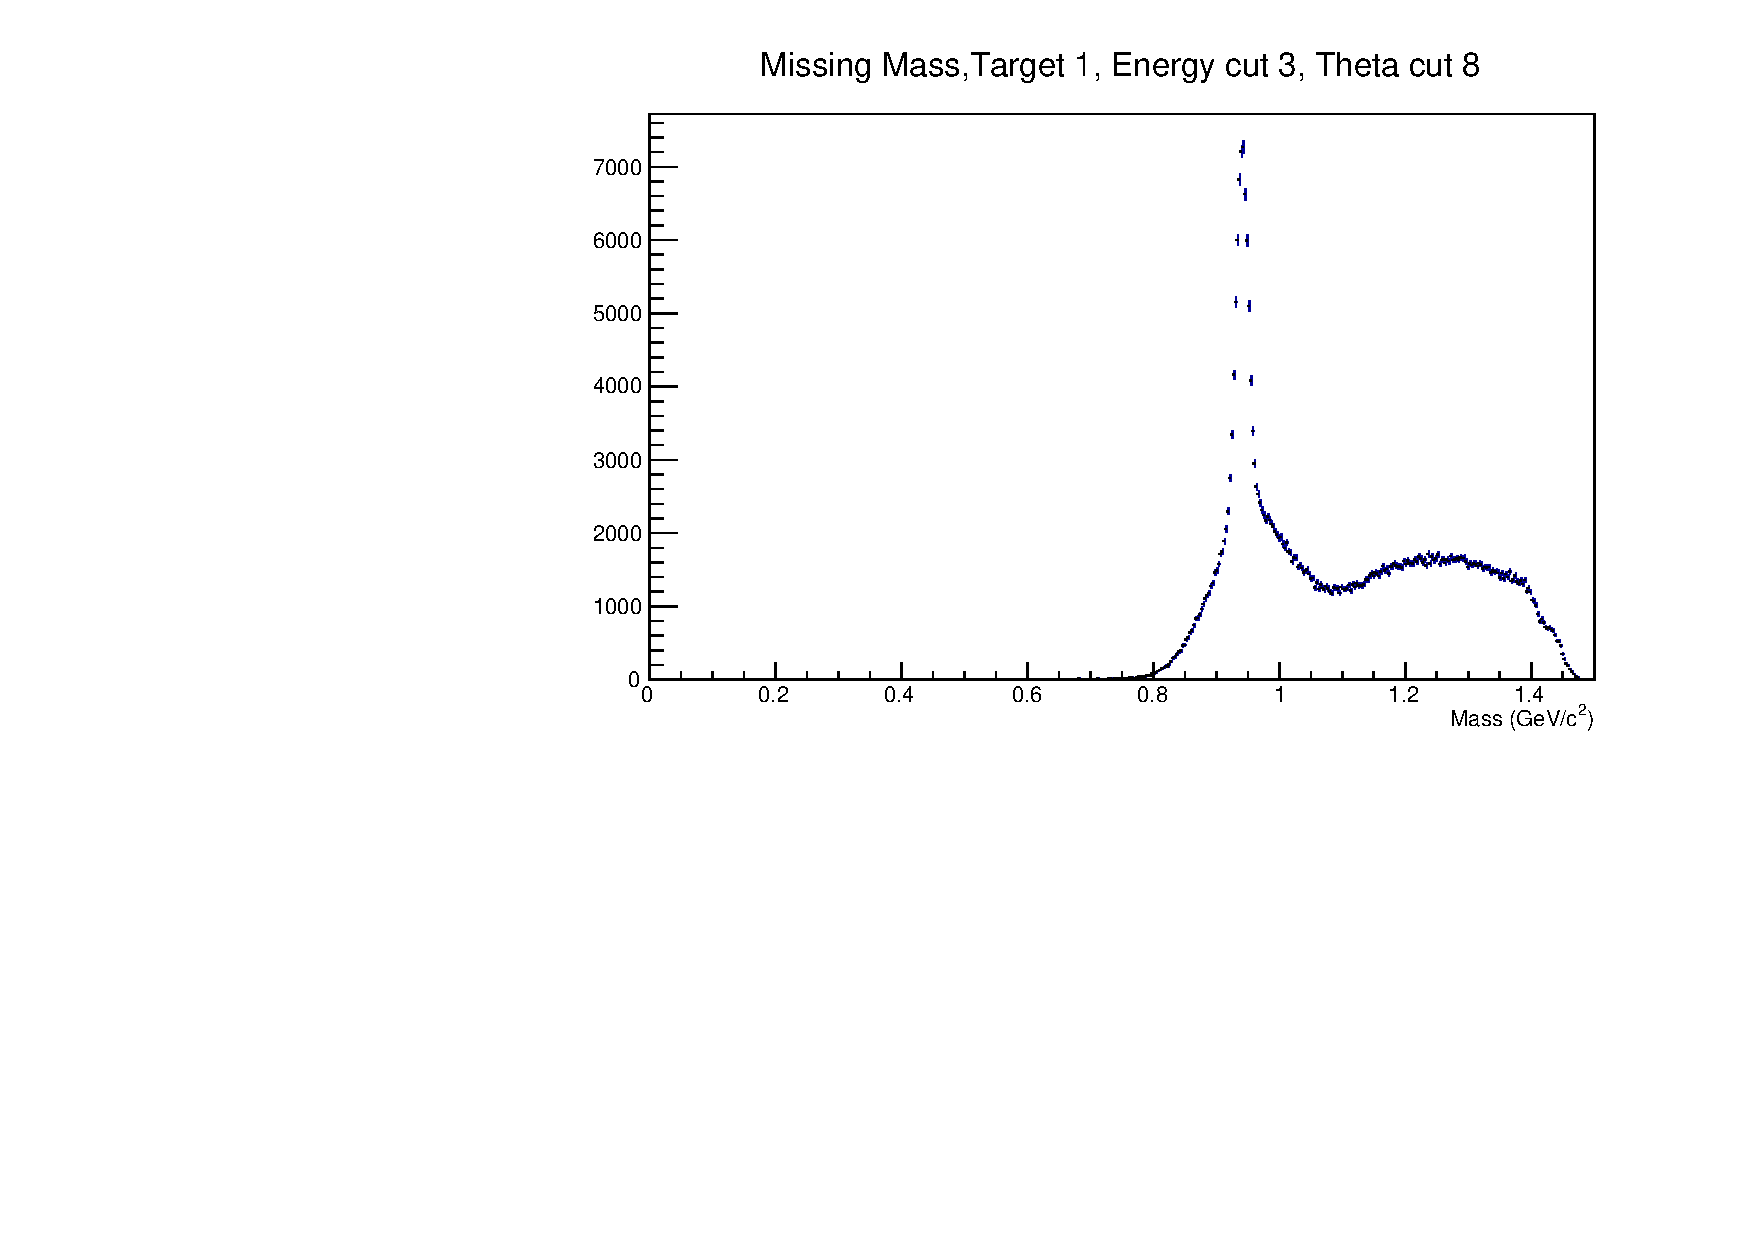
\includegraphics[width=0.6\textwidth]{figures/neutron_missingmass.pdf} \\
    \caption{Mass distribution obtained from the reconstructed neutron four-vector, displaying a sharp peak corresponding to the reconstructed neutron and
a broad peak to the right of this corresponding mainly to two-pion production channels. }
    \label{fig:frost_neutronmissing_ex}
  \end{center}
\end{figure}
\begin{figure}[H]
  \begin{center}
    \includegraphics[width=0.6\textwidth]{figures/scaling_dilutionfactor.pdf} \\
    \caption{Fitting of the ratio of butanol missing mass distribution with carbon missing mass distribution. The function used is a Gaussian plus a zeroth order polynomial: The zeroth order polynomial will give the constant scaling factor for the carbon target missing mass distribution. }
    \label{fig:scaling_dilutionfactor}
  \end{center}
\end{figure}
Fig. \ref{fig:frost_neutronmissing_ex} shows an example of the missing mass distribution obtained from the reconstructed neutron four-vector in the butanol target, showing a sharp peak corresponding to the missing neutron mass and a broad peak to the right of this corresponding to other possible channels such as multi-pion production. This plot also shows background contributions due to photon interactions with the carbon and oxygen atoms in the butanol target.
A missing mass cut was applied to select the mass region containing the $p(g,\pi^+)n$ events of interest: Following the systematic study on the width of the missing mass cut done by S. Strauch in \cite{Strauch_2014} a cut of $2 \sigma$ around the neutron missing mass was used in each bin \footnote{This cut was established from the data after the nuclear subtraction described below}. \\
Even with the mass cut described above the selected yield will contain events arising from $\pi^+$ production on the unpolarised nuclei in the butanol (Carbon and Oxygen). The shape of the unpolarized background was established using the data from the carbon target. 
 The missing-mass distribution obtained from the carbon target was first scaled to the butanol missing-mass distribution. To obtain the scale factor (i.e. the fraction of unpolarized data in the yield), the ratio of the  missing mass spectrum for butanol and carbon were fitted with a Gaussian function and a zeroth order polynomial (an example fit  is shown in Fig. \ref{fig:scaling_dilutionfactor}). The gaussian peak is from the $p(\gamma,\pi^+)n$ events in the butanol and the zeroth order polynomial gives the scaling factor for the contribution of unpolarized events in the region around the neutron peak. \\
A distinct hydrogen contamination was observed for the face of the carbon target farther from the butanol (see Fig. \ref{fig:dilution_factor_z0}) attributed to a thin layer of ice formed on the target surface. Therefore a cut was applied to the MVRT.Z position for each beam configuration in order to remove the "face" region where the hydrogen contamination is most significant (See Table \ref{table:dil_factor_zcut}) \footnote{This approach was seen as more consistent for all different bins and settings than using a double fitting procedure for removing the main part of the hydrogen contamination}. For this "cleaned" data set was performed a fit on the missing mass distribution using a combination of a Gaussian function and a third order polynomial (See Fig. \ref{fig:dilution_mass_zcut}). The Gaussian function represented the (Fermi smeared) neutron peak due to the quasi-free pion photoproduction from the carbon and oxygen nuclei. The polynomial modeled the broad background coming from mostly multi-pion production and other non-quasi-free processes.  A lower limit was set for the $\sigma$ of the Gaussian function, using the value for the same parameter obtained from the butanol target\footnote{As the carbon and butanol targets were very close together in the beamline they could not be fully resolved in the z-vertex distribution spectrum for certain $cos(\theta_{CM})$ (mainly forward and backward angles due to poor reconstruction from the MVRT bank) bins, some events for those bins within the carbon z-vertex cuts will have originated from polarized protons within the butanol target.} (See Fig. \ref{fig:dilution_mass_zcut}). The integral of the butanol experimental data in the neutron mass peak gave $N_B$. For the carbon background the results from fitting to the normalized carbon data was used to evaluate $N_C$, by integrating this function over the neutron missingmass region.  The dilution factor to be calculated as:
\begin{equation} \label{eqn:dil_factor}
  D_F = \frac{N_B - N_C}{N_B}
\end{equation}
 For the butanol data the statistics for each bin were high enough to derive the statistical error in $N_B$ from the Integral of the yield in the $2\sigma$ missing mass region. For the error on $N_C$, in order to keep a conservative approach for both ranges ($W<1.8GeV$ and $W\geq 1.8GeV$) , the histogram Integral error was used, since it better reflects the statistical uncertainties of each bin and  does not introduce any model dependency because does not come from a fitting procedure \footnote{This was done so that low statistics bins where the fit was not well defined would have an appropriate error. Fig. \ref{fig:dilution_fit_comp2} shows an example case where the shape of the carbon background indicates inconsistency with neighboring energy bin (shown by the difference between the two lines on the figure). }. Figs \ref{fig:dilution_comp_E0} to \ref{fig:dilution_comp_E3} show examples for a range of photon energy bins  of butanol missingmass spectra  compared to the scaled carbon data, along with the fit (red line) used to establish the carbon yield $N_C$. The extracted dilution factors (obtained from equation \ref{eqn:dil_factor}) are presented as a function of W for a single $cos(\theta_{CM})$ bin in Fig. \ref{fig:dilution_fit_theta6}. The result of the fit was then fitted with a linear function in the region $W>1.8GeV$ in order to minimize fluctuations due to poor statistics.
 
\begin{figure}[H]
  \begin{center}
    \subfloat[][Carbon missing mass spectrum (X(GeV)) vs MVRT.Z position (Y(cm))] {
      \includegraphics[width=0.64\textwidth]{figures/mvrt_cut_dilution_factor_1_1.pdf} 
      \label{fig:dilution_factor_z1}
    }
    \qquad
    \subfloat[][Carbon missing mass spectrum in GeV for 5.7cm $<$ MVRT.Z $<$ 6.2cm] {
      \includegraphics[width=0.32\textwidth]{figures/mvrt_cut_dilution_factor_1.pdf}
    \label{fig:dilution_factor_z2}
    }
    \qquad
    \subfloat[][Carbon missing mass spectrum in GeV for 6.8cm $<$ MVRT.Z $<$ 7.3cm] {
      \includegraphics[width=0.32\textwidth]{figures/mvrt_cut_dilution_factor_2.pdf}
    \label{fig:dilution_factor_z3}
    } 

    \caption{\ref{fig:dilution_factor_z1}The missing mass spectrum is plotted for the carbon target as a function of the reconstructed z vertex in the target (extracted from MVRT bank). The missing mass distribution after selection on large z ( to emphasize the hydrogen (ice) contamination) is shown in Fig. \ref{fig:dilution_factor_z3}, which illustrates the narrow peak having width and properties consistent with hydrogen data. For comparison Fig.  \ref{fig:dilution_factor_z2}  shows the missing mass for a more central region of the graphite where little evidence of hydrogen contamination is evident.}
    \label{fig:dilution_factor_z0}
  \end{center}
\end{figure}

\begin{table}
  \begin{center}
    \begin{tabular}{ ||l|r|r|r|r|r|r|r|r|r||}
      \hline
      \multicolumn{10}{|c|}{g9a Run period: Linearly polarized } \\
      \hline
      $Coh_{Edge}$(GeV)&0.73&0.93&1.1&1.3&1.5&1.7&1.9&2.1&2.3 \\
      \hline
      $Z_{cut}$(cm)&6.1&6.1&6.2&6.2&6.2&6.4&6.4&6.4&6.5 \\
      \hline
    \end{tabular}
  \end{center}
  \caption{g9a Run period: The photon energies corresponding to the Coherent Edge ($Coh_{Edge}$) are shown together with the MVRT.Z upper limit used in order to avoid the ``face'' where hydrogen contamination (probably ice) is strongly evident. See Fig. \ref{fig:dilution_factor_z0}.}
  \label{table:dil_factor_zcut}
\end{table}

\begin{figure}[H]
  \begin{center}
    \includegraphics[width=0.8\textwidth]{figures/plot_dil_730_tot_E1_theta6.png} \\
    \caption{Missing Mass distribution for the carbon target before (BLUE) and after(RED) the Z vertex cut. The cut histogram (RED) is scaled to the uncut (BLUE) in the region M=0.9-1.2GeV, outside the region where hydrogen data would be expected to contribute. The red line shows a fit to the cut data comprising a gaussian plus a 3rd order polynomial. The gaussian width in the fit has minimum value constrained by the same fit to the butanol data.  
 For the error on the carbon subtraction, I have used the area delimitated by the statistical error of each bin in the carbon histogram in the range where the butanol missing mass is considered (in this bin the $-2\sigma$ to $2\sigma$ range includes values from 0.91GeV to 0.97GeV).}
    \label{fig:dilution_mass_zcut}
  \end{center}
\end{figure}


\begin{figure}[H]
  \begin{center}
    \subfloat[][Energy Cut 1] {
      \includegraphics[width=0.25\textwidth]{figures/plot_dil_1300_tot_E0_theta6.png} 
      \label{fig:dilution_comp_E0}
    }
    \subfloat[][Energy Cut 2] {
      \includegraphics[width=0.25\textwidth]{figures/plot_dil_1300_tot_E1_theta6.png}
    \label{fig:dilution_comp_E1}
    }
    \subfloat[][Energy Cut 3] {
      \includegraphics[width=0.25\textwidth]{figures/plot_dil_1300_tot_E2_theta6.png}
    \label{fig:dilution_comp_E2}
    }
    \subfloat[][Energy Cut 4] {
      \includegraphics[width=0.25\textwidth]{figures/plot_dil_1300_tot_E3_theta6.png}
    \label{fig:dilution_comp_E3}
    } \\
    \subfloat[][Dilution factor vs W for  $ 0.2 <= cos(\theta_{CM})<0.4$] {
      \includegraphics[width=0.5\textwidth]{figures/comp_DF_TGPOL_system_6.png}
      \label{fig:dilution_fit_theta6}
      }
    \subfloat[][Comparison of fitted carbon Missing mass distribution] {
      \includegraphics[width=0.5\textwidth]{figures/dilution_factor_1300_E1_E2_theta6_comp2.pdf}
      \label{fig:dilution_fit_comp2}
      }
    \caption{Missing Mass distribution for butanol (BLUE) and carbon(RED) after the Z vertex cut (Carbon Target cut and ice removal defined in Tab. \ref{table:dil_factor_zcut}) for the carbon target. A fitted function (RED line)  is used to smooth the carbon missing mass distribution (a Gaussian plus a polynomial of 3-rd order). This bin corresponds to the Coherent edge of 1.3GeV (This data-set has been divided into 4 W bins; For this settings, the contribution for butanol in the missing mass spectrum (and so for the dilution factor) is considered just in the range from $\sim 0.88$ GeV to $\sim 0.99$ GeV). The W dependence for this data set is shown in see Fig. \ref{fig:dilution_fit_theta6} and the highlighted region shown by the box indicates the data extracted from the fits in Fig. \ref{fig:dilution_comp_E0},\ref{fig:dilution_comp_E1},\ref{fig:dilution_comp_E2},\ref{fig:dilution_comp_E3}.
      In Fig. \ref{fig:dilution_fit_comp2} it is plotted Fig.\ref{fig:dilution_comp_E0} together with the scaled carbon fitted function for the adjacent energy bin.  }
    \label{fig:dilution_fit_comp}
  \end{center}
\end{figure}

The Dilution factor shows some W dependent structure for $W < 1.8GeV$, especially for central $\theta_{CM}$. Similar structure was seen in the previous analysis by S. Strauch in \cite{Strauch_2014} that used circularly polarized photon beam \footnote{Keeping into consideration that in this previous analysis, with a better photon resolution (and therefore missing mass resolution) due to lower electron beam energy, the dilution factor was higher than the one calculated here}. Such structures would be expected due to different W dependence of the cross sections for pion photo-production from the proton and nuclei (see as example Fig. \ref{fig:comparison_dilutionfactor}). It is well established that the strong resonance structure observed on the proton in the second resonance region above the $\Delta$  is largely washed out in pion production from nuclei, so it would be expected to influence the extracted dilution factor which is formed from the ratio of nuclear and proton yields. For $W \geq 1.8GeV$, above the strong second resonance region, the Dilution factor it is not expected to show significant structure: For this reason, a linear fit to the dilution factor data was used for this mass range to smooth statistical fluctuations. Although the dilution factor used the fitted line to give values in each bin, the statistical error in the dilution factor data for each bin was used in estimating the error. Two different fits have been used in order to take into account the different neutron mass resolutions observed for the data settings having different electron beam energies (indicated by the colour coding of the data points in Fig\ref{fig:comparison_dilutionfactor}). The extracted dilution factors for each $cos(\theta_{CM})$ bin are shown in  appendix \ref{app:dilfactor} from page \pageref{app:dilfactor}.  

\begin{figure}[H]
  \begin{center}
    \includegraphics[width=0.6\textwidth]{figures/comp_DF_maid_crosssection.pdf} \\
    \caption{Dilution factor for a single $cos(\theta_{CM})$ bin vs W (RED, GREEN, BLUE points correspond to electron beam energy settings of 2.780GeV, 1.545GeV and 4.599GeV respectively). Also plotted for comparison is the scaled total cross section for $\pi^+$ photoproduction on proton from the MAID 2007 model \cite{MAID_2007} (BLACK points). For $W \geq 1.8GeV$ a linear fit is used for the two electron beam energy settings in this range in order to mitigate possible fluctuations in the extraction of G.}
    \label{fig:comparison_dilutionfactor}
  \end{center}
\end{figure}


\subsection{Calculation of Systematic Corrections and Systematic error evaluations used in  the extraction of G and \texorpdfstring{$\Sigma$}{Sigma}}
\label{ch:sys_corr}
In this section we will describe how the systematic errors for the results were obtained and how necessary systematic corrections were evaluated and applied. A key part of this assessment was the development of a model for simulating the extraction of G and $\Sigma$. This study  quantifies any necessary systematic corrections induced by the extraction process. A simulation of the reaction process was developed in which the photon energy dependence of the photon polarization, statistics, and target polarization can be varied and the effects on the G,$\Sigma$ extraction can be assessed. As a basis, the real distributions obtained by the data (bin-by-bin) were input to the model. In this way we could address possible sources of systematic effects and improve our extraction method. \\ 
In the study all parameters contributing to the cross section (equation \ref{eqn:extract_G_S}) were tested to explore their systematic sensitivities to the extraction of G and $\Sigma$. The studies carried out are listed below with the results outlined in the following sections.

\begin{enumerate}
\item Photon Polarization ($P_{\gamma}$) (see chapter \ref{sec:ph_pol_sys} for more details) was tested for:
  \begin{enumerate}
  \item different photon energy dependences for the photon polarization for the $cos(\theta_{CM})$,W bin,
  \item combining data with different coherent edge settings for the photon beam,
  \item varying the beam polarization around the actual value with a random error.
  \end{enumerate}
\item Target Polarization ($P_z$) (see chapter \ref{sec:tg_pol_sys} for more details) was tested for
  \begin{enumerate}
  \item Different time dependence of the polarization during the data taking for the $cos(\theta_{CM})$,W bin,
  \item combining data with different coherent edge settings.
  \end{enumerate}
\item Since the extraction of G and $\Sigma$ is correlated (see  equations \ref{eq:N1} - \ref{eq:N4}) a grid of 11 different values for G and $\Sigma$ was simulated (see section \ref{sec:G_Sigma_sys} for more details)
\item Different statistics in the same $cos(\theta_{CM})$,W bin for Parallel and Perpendicular photon polarization and Amorphous radiator runs: As expected no extra source of systematic errors (that is not already described by the correction defined at \ref{sec:G_Sigma_sys}) comes from this effect. 
\item Two different ways of filling the $\phi_{\pi^+}$ histograms have been tested (see section \ref{sec:weighthisto} for more details):
  \begin{enumerate}
  \item Filling the histograms without any weighting (I will use equation \ref{eq:N1} - \ref{eq:N4} in order to extract G and $\Sigma$)
  \item Filling the histograms with a weight of $(1/P_{\gamma})$ in order to try to normalize the weight of different events with different Photon polarization  $P_{\gamma}$ (I will need to modify equation \ref{eq:N1} - \ref{eq:N4}, see chapter \ref{sec:weighthisto} and \ref{ch:extract_G_S} for details) .
  \end{enumerate}
\end{enumerate}
Analyzing the results of these simulations (see Appendix \ref{app:simcode} for a sample of the code used) gave some interesting insights on how to address the analysis of the data. These are discussed in the following sections.


\subsubsection{Photon Polarization}\label{sec:ph_pol_sys}
For the photon polarization, the effect on the extracted G and $\Sigma$ when using modified shapes for the variation of polarization with e-gamma \footnote{The starting point the actual  data profile for the Beam polarization histogram for each $W$, $cos(\theta_{CM})$ bin} and also including a gaussian error on the polarization (with sigma taken from the statistical error in the determination of the coherent edge position) have been tested. None of these studies (carried out separately for each costheta, W bin) yielded systematic changes of the extracted values of G and Sigma greater than 1\%. The dominant systematic in the photon polarization therefore comes from the theoretical modelling (including account of the beamline parameters) required to relate the coherent edge positions to the polarization. The quoted systematic error for this procedure (obtained from colleagues at Glasgow who carry out these calculations) is 10\%.
 This systematic error was added in quadrature to the Polarization statistical error obtained from the polarization tables \cite{Anderson_table}. \\
Systematic effects on the Photon Polarization from only keeping the photons where the polarization is predicted to be $>50\%$  have been checked by varying the selection of the allowed range around the nominal value of $>50\%$. The different selections employed in this study are listed below: 
\begin{align}
  P_\gamma &> 45 \% \\
  P_\gamma &> 50 \% \\
  P_\gamma &> 55 \% 
\end{align}
In most cases this was a negligible effect. However for some $W$. $cos(\theta_{CM})$ bins where the photon energy corresponds to the extremities of the coherent peak range some small variations were noted. These bins are shown when presenting the final results (sections \ref{ch:result_W} and \ref{ch:result_th} where this effect is shown as a generally small increased error (the error including this effect is shown by the \color{red}{red} \color{black}{error} bars, without this effect by the black error bars). 


\subsubsection{Target Polarization}\label{sec:tg_pol_sys}
The Target polarization was slowly varying through the experimental data taking, typically at a rate around 1\% per day \cite{Keith_2012}. The values for the target polarization, averaged over the beamtime for each coherent edge setting are shown in the appendix (chapter \ref{app:tgpol}).  Analysis of simulated data showed that the decay of the target polarization does not affect the extraction of G and $\Sigma$, within an error below 1\%. As in the previous study this was assessed on a bin-by-bin basis in $W$, $cos(\theta_{CM})$. \\
The simulation analysis also showed that (as expected \footnote{This is as in the analysis the product $G,P_z$ is extracted from an offset in the $\phi$ distributions from zero. Data with significantly different degrees of target polarization would mean merging data with different $\phi$ offsets.}) combining data sets with significantly different degrees of target polarization would produce unwanted systematics in the extraction of G and $\Sigma$. Therefore we analyze the different target polarization settings separately. 

  
\subsubsection{Dependence of G and \texorpdfstring{$\Sigma$}{Sigma} extraction on the  statistics of the W, theta bin}\label{sec:G_Sigma_sys}
The extraction of G and $\Sigma$ from the data is correlated and our simulation showed that the extracted values of G and Sigma showed some variations from the values set in the simulation, when dealing with bins having low statistics.  For this reason, these 3 variables (G, $\Sigma$, $N_{ev}$) were investigated with multiple simulations that covered the full range of the experimental data. A systematic shift between the true and extracted values was seen for the extracted values of G and $\Sigma$ for $W$, $cos(\theta_{CM})$ bins. This correctione becomes relevant when statistics goes below 3000 events. In this region, and in the full range of G and $\Sigma$, multiple simulations (100 simulations) were done with the same settings (G,$\Sigma$, number of events) in order to mitigate statistical fluctuations and establish a set of Systematic corrections.  \\
The averaged systematic correction was then extracted for the same number of events as the data in the experimental bins (see Fig. \ref{fig:sys_correction_100} for an example). For each calculated value of G and $\Sigma$, an interpolated systematic correction for a given statistics in the bin was calculated (See Fig. \ref{fig:calc_sys_correction}). 
This procedure was carried out over the full range of sample sizes per $W$, $cos(\theta_{CM})$ (the sample sizes were chosen to cover the ranges seen in the experimental data, corresponding to statistics up to 3000 events). Interpolating between these data allowed the correction to be evaluated for any G,$\Sigma$,$N_{Ev}$ combination. The correction was evaluated bin-by-bin and applied to the extracted results for G and $\Sigma$ from the experimental data.  \\
A full picture of the systematic correction for G and $\Sigma$ obtained from the simulation is shown in the appendix (see chapters \ref{app:G_syscorr} and \ref{app:Sigma_syscorr}). It is interesting to see how the correction changes sign and increases rapidly in magnitude when the statistic of the events goes below a certain threshold. The statistics at each beam was kept where possible with counts above 3000 in order to introduce not negligeble systematic effects. Where the statistic was below 3000 events, the systematic correction was applied . 
Similar bin statistical effects were observed and correction were applied when extracting $\Sigma$ from CLAS data (e.g. \cite{Zacha_2017}). The existence of the effect in this case was put down to fitting a function to binned data. Similar effects are expected in our case with the added correlation of the contemporary extraction of G and $\Sigma$.
\begin{table}
  \begin{center}
    \begin{tabular}{ ||c|c|c|c|c|c|c|c|c|c|c|c|c|c||}
      \hline
      \multicolumn{14}{|c|}{Number of Events ($N_{ev}$) simulated for the full G (11 points) and $\Sigma$ range (11 points)  } \\
      \hline
      \hline
      50&60&70&80&90&100&110&120&130&140&150&160&170&180\\
      \hline
      190&200&250&300&350&400&500&600&700&800&900&1000&2000&3000 \\
      \hline
    \end{tabular}
  \end{center}
  \caption{Number of events simulated for each combination of G and $\Sigma$ in order to get a full evaluation of the systematic correction dependence as a function of the statistic available at each $W$,$cos(\theta_{CM})$ bin}
  \label{table:sim_nevents}
\end{table}


\begin{figure}[H]
  \begin{center}
    \includegraphics[width=0.6\textwidth]{figures/Sys_corr/Graph_G_100.pdf} \\
    \caption{Systematic correction for G with a statistic of 100 events as a function of the extracted values for G and $\Sigma$. Each combination of G and $\Sigma$ is simulated 100 times and averaged after extraction of the parameters. }
    \label{fig:sys_correction_100}
  \end{center}
\end{figure}
\begin{figure}[H]
  \begin{center}
    \includegraphics[width=0.6\textwidth]{figures/Sys_corr/calc_correction.pdf} \\
    \caption{Systematic correction for G with its error for a fixed G=0.42 and $\Sigma$=0.24. The error is presented as a  as a function of the statistic for the $W$,$cos(\theta_{CM})$ bin (For a list of the different statistic used, see Table \ref{table:sim_nevents}).  }
    \label{fig:calc_sys_correction}
  \end{center}
\end{figure}

\subsubsection{Weighting while filling the histograms} \label{sec:weighthisto}
Two different ways of filling the $\phi_{\pi^+}$ distribution histograms before fitting to extract G and Sigma were explored. Two methods were studied:
\begin{enumerate}
\item the average photon polarization for the bin is evaluated and applied to the extracted G, $\Sigma$, 
\item  a weighting method where the polarization is accounted for event by event.
\end{enumerate}
 The filling of the histograms with a weight of $(1/P_{\gamma})$ was tested in order to try to normalize the weight of different events with different Photon polarization  $P_{\gamma}$, considering also the associated error in the extracted value of the Polarization. Results were compared for different statistics, and method 2 (weighted version) gave more stable results, giving less fluctuations in response to changes in the statistics within the bin. \\
In order to propagate the error correctly while filling the histogram with the weight of $(1/P_{\gamma})$, the default method in ROOT was modified, since it does not consider an error carried by the weight.
Each event (see the simulation code at chapter \ref{app:simcode} from line 76 to 86) recorded was filled following the default function from ROOT. For the error associated with each event, both the error carried by the statistic of adding each event in a bin ($\sigma_{ev} = 1$) and the error carried by the weight (in this case, the beam polarization) were accounted for. The procedure used to fill the histograms is described below 
\begin{align}
  Bin_{err} = & histo\rightarrow GetBinError(bin) &  \textnormal{the error is  got before filling the bin} \\
  &  histo\rightarrow Fill(\phi,1/P) & \textnormal{histogram is filled with the weight of}\, 1/P \\
  Value_{err} = & \sqrt{\frac{\sigma_{ev}^2}{P^2} + \frac{\sigma_P^2}{P^4}} & \textnormal{error for this event, where}\, \sigma_{ev}=1 \\
  New_{err} = & \sqrt{Bin_{err}^2 + Value_{err}^2} & \textnormal{calculating the new error for this bin}
\end{align}

It was found that using method (1) or method (2) gave consistent results within 1\% (after averaging between trials). Since it showed less dependence on bin statistics, method (2) is subsequently used in the analysis of the data \footnote{with the exception of one beam setting ($0.730 GeV$) where the coherent edge data was not correctly recorded in the EPICS bank during the run, and accumulated data for the beam polarization was needed to be use}.



\subsection{Contemporaneous extraction of G and \texorpdfstring{$\Sigma$}{Sigma} from the experimental data} \label{ch:extract_G_S}
In this section the fits applied to extract G and $\Sigma$ from the experimental data are outlined.  After the flux normalization, and the use of the weighted method for inputting the beam polarization weighted (by $1/P_{\gamma}$) histograms, the new $\phi$ distribution will update equations \ref{eq:N1} - \ref{eq:N4} into:
\begin{eqnarray}
N_{\parallel +} = A_{NORM} \left( \frac{1}{P_{\gamma \parallel}} + \Sigma cos(2(\phi-\phi_0)) +  P_{+z\parallel} G sin(2(\phi-\phi_0)) \right) \label{eq:UN1}\\
N_{\parallel -} = A_{NORM} \left(\frac{1}{P_{\gamma \parallel}} + \Sigma cos(2(\phi-\phi_0)) - P_{-z\parallel} G sin(2(\phi-\phi_0)) \right) \label{eq:UN2}\\
N_{\perp +} = A_{NORM} \left( \frac{1}{P_{\gamma \perp}} - \Sigma cos(2(\phi-\phi_0)) -  P_{+z\perp} G sin(2(\phi-\phi_0)) \right) \label{eq:UN3}\\
N_{\perp -} = A_{NORM} \left( \frac{1}{P_{\gamma \perp}} - \Sigma cos(2(\phi-\phi_0)) +  P_{-z\perp} G sin(2(\phi-\phi_0)) \right) \label{eq:UN4}\\
\end{eqnarray}
In order to remove the remaining effects due to acceptance and to allow the simultaneous extraction of G and $\Sigma$ combining the statistics from the PARA and PERP measurements, an asymmetry was constructed, $A(\phi)$ (shown below for the case of positive target polarization $P_{+z}$),
\begin{equation}
  A(\phi)_+ = \frac{N_{\parallel +} - N_{\perp +}}{N_{\parallel +} + N_{\perp +}} = \frac{ (\frac{1}{P_{\gamma \parallel}} - \frac{1}{P_{\gamma \perp}}) + 2 \Sigma cos(2(\phi-\phi_0)) +  (P_{+z\parallel}+P_{+z\perp}) G sin(2(\phi-\phi_0))}{(\frac{1}{P_{\gamma \parallel}} + \frac{1}{P_{\gamma \perp}}) +(P_{+z\parallel}-P_{+z\perp}) G sin(2(\phi-\phi_0))} \label{eq:A1}
\end{equation}
\begin{figure}[H]
  \begin{center}
    \subfloat[][Asymmetry for $1.71GeV \leq E_{CM} < 1.74GeV$ and $0.4 \leq cos(\theta_{CM}) < 0.6$  ] {
      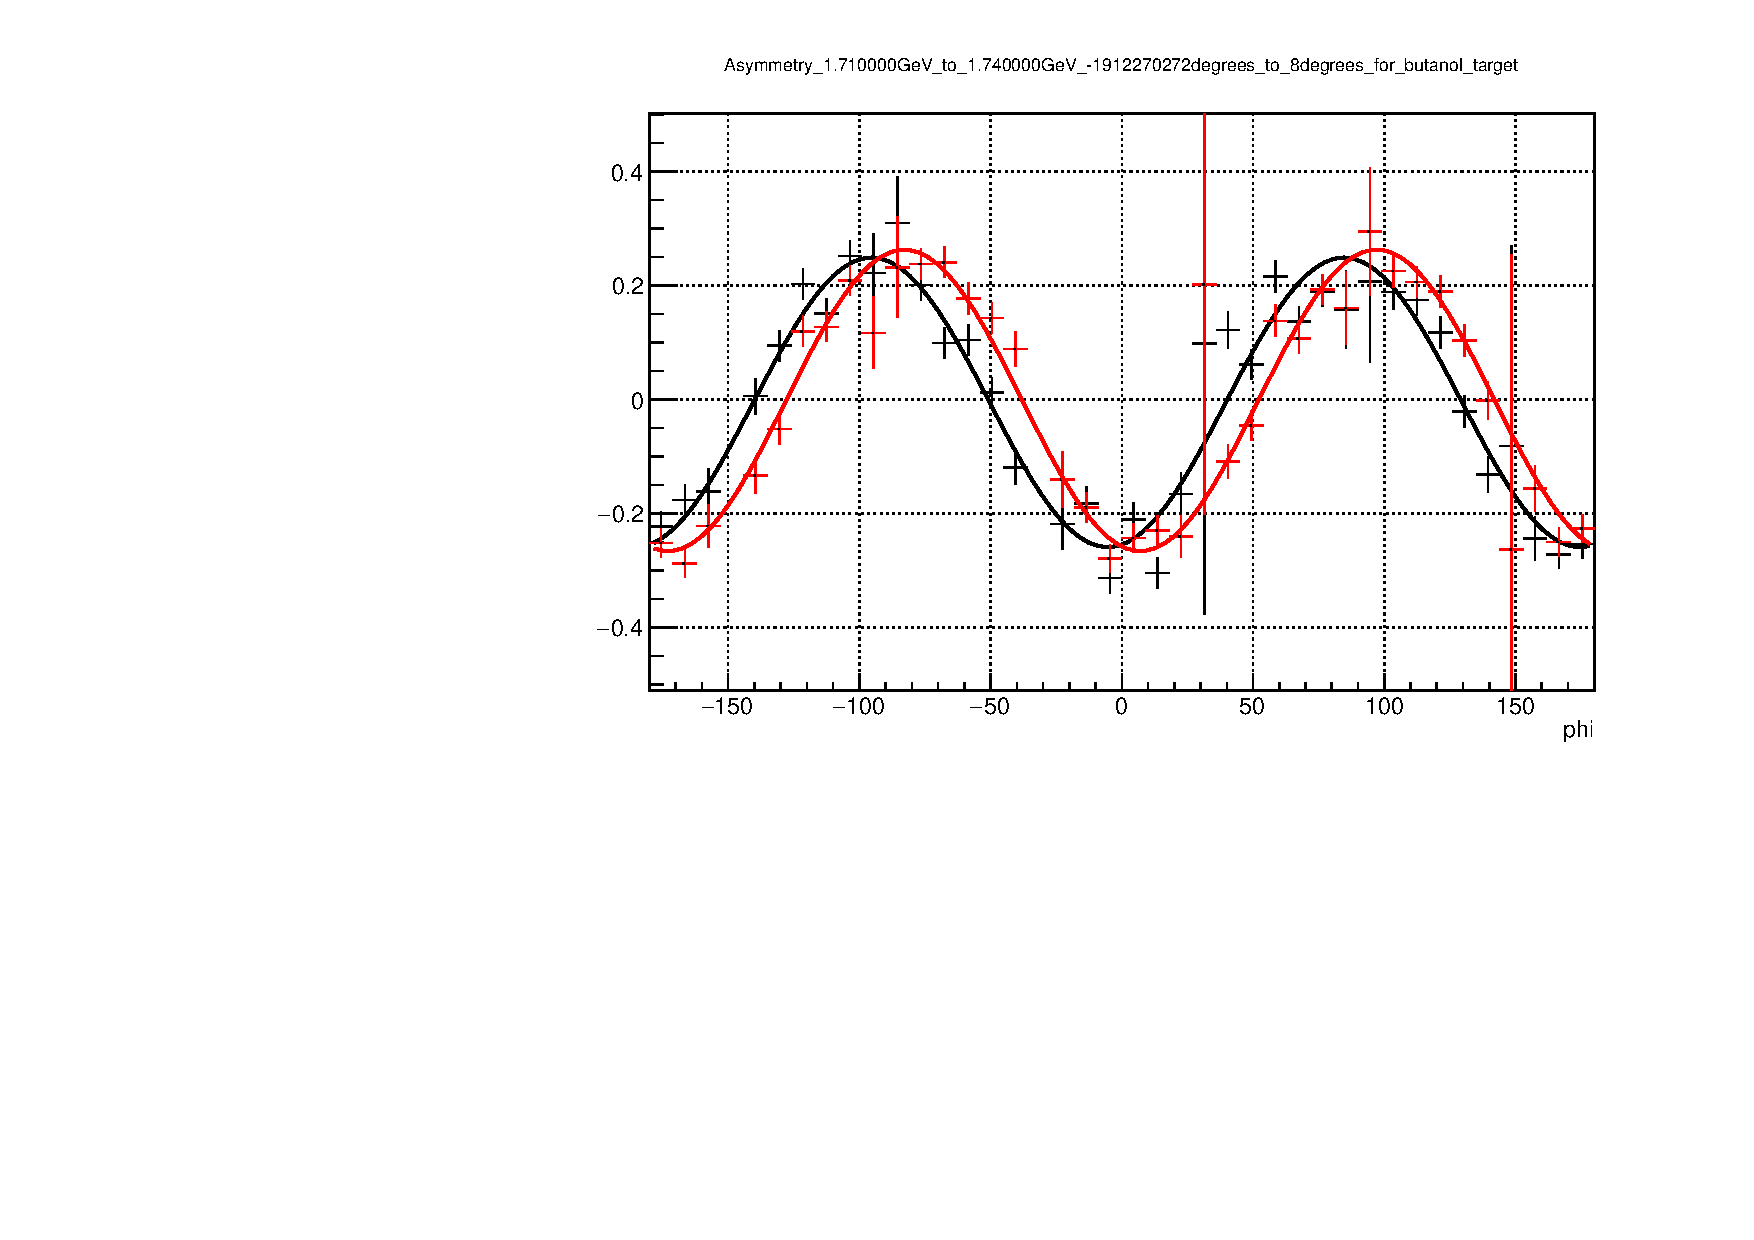
\includegraphics[width=0.9\textwidth]{figures/G_tgpol_effect.pdf} 
      \label{fig:GTgpol_theta1}
    }
    \caption{The Asymmetry histogram with the fit is plotted for the two different target polarization. One can see the expected symmetric shift from the center ($\phi = 0$) for the different polarizations.  }
    \label{fig:GTgpol}
  \end{center}
\end{figure} 
During the experimental data-taking PARA,PERP and AMO configurations were switched regularly during the same day (the change in $P_z$ is $\sim 1\%$ in a day). If data with the same $W$,$cos(\theta_{CM})$ bin was taken at different periods (which could have different $P_z$), the results were extracted separately (if statistically valuable). This allow us to safely consider for the target polarization
\begin{equation}
  (P_{+z\parallel}-P_{+z\perp}) \ll 1 \% 
\end{equation}
One can also use the harmonic mean ($\bar{p}$)for the PARA and PERP configurations of the photon polarization in order to further simplify equation \ref{eq:A1} 
\begin{equation}
  \frac{2}{\bar{p}} = \left(\frac{1}{P_{\gamma \parallel}} + \frac{1}{P_{\gamma \perp}}\right)
\end{equation}
Applying these two equations, one can obtain a simplified version for the created asymmetry
\begin{equation}
  \frac{N_{\parallel +} - N_{\perp +}}{N_{\parallel +} + N_{\perp +}} = \left( (\frac{1}{P_{\gamma \parallel}} - \frac{1}{P_{\gamma \perp}}) + 2 \Sigma cos(2(\phi-\phi_0)) +  (P_{+z\parallel}+P_{+z\perp}) G sin(2(\phi-\phi_0)) \right) \frac{\bar{p}}{2} \label{eq:A2}
\end{equation}
A fitted function was used in order to extract the values (after testing that $\phi_0$ was statistically consistent with 0, the parameter was fixed in order to remove unnecessary fit parameters):
\begin{align}
  f(\phi) & = A + B cos(2(\phi-\phi_0)) + C sin(2(\phi-\phi_0)) \\
  \Sigma & = \frac{B}{D_F \, \bar{p}} \\
  G & = \frac{C}{D_F \, \bar{p} \,\bar{p_z}} \\
    \textnormal{where:} \, D_F & =   \textnormal{Dilution Factor} \\
    \bar{p_z} & =  \frac{P_{+z\parallel}+P_{+z\perp}}{2}
\end{align}
The results are obtained (See for example Fig. \ref{fig:GTgpol}) separately for both target polarizations. These gave statistically consistent results (See appendix at \ref{app:G_TGPOL} and at \ref{app:Sigma_TGPOL}). The final results come from a weighted average of the G or $\Sigma$ extracted from the two target polarizations. These results are presented in the next chapter.



